\documentclass[10pt]{beamer}

\usetheme[progressbar=frametitle]{metropolis}
\usepackage{appendixnumberbeamer}

\usepackage{booktabs}
\usepackage[scale=2]{ccicons}

\usepackage{pgfplots}
\usepgfplotslibrary{dateplot}

\usepackage[boxed,ruled]{algorithm}
\usepackage{multirow}
\usepackage{algpseudocode}
\usepackage[sort&compress]{natbib}

\usepackage{xspace}
\newcommand{\themename}{\textbf{\textsc{metropolis}}\xspace}

\title{Hierarchical-block conditioning approximations for high-dimensional multivariate normal probabilities}
% \subtitle{A modern beamer theme}
\date{\today}
% \date{}
\author{Hyunseok Yang, Kyeongwon Lee, and Songhyun Kim}
\institute{Department of Statistics, SNU}
% \titlegraphic{\hfill\includegraphics[height=1.5cm]{logo.pdf}}

\begin{document}

\maketitle

\begin{frame}{Table of contents}
  \setbeamertemplate{section in toc}[sections numbered]
  \tableofcontents%[hideallsubsections]
\end{frame}

% intro
\section{Introduction}

\begin{frame}{\secname}

    \begin{itemize}
        \item The computation of the multivariate normal (MVN) probability 
        \begin{equation}\label{eqn:normalprob}
            \Phi_n(\mathbf{a}, \mathbf{b}; 0, \boldsymbol{\Sigma}) = \int_a^b \frac{1}{\sqrt{(2\pi)^n |\boldsymbol{\Sigma}|}} \exp\left( -\frac{1}{2} \mathbf{x}^T \boldsymbol{\Sigma}^{-1} \mathbf{x} \right) d\mathbf{x},
        \end{equation}
        where $\mathbf{a}$ and $\mathbf{b}$ are integration limits, the mean vector $\mu$ is assumed to be 0, $\boldsymbol{\Sigma}$ is a positive-definite covariance matrix, is required for a variety of applications. 
        \item Various methods to compute MVN probability are suggested such as Richtmyer Quasi-Monte Carlo(QMC) \citep{genz2009computation}
        \item However, In high-dimensional settings (large $n$), it is hard to compute \eqref{eqn:normalprob} directly.
        \item We review new approaches proposed by \citet{cao2019hierarchical} to approximate high-dimensional multivariate normal probability \eqref{eqn:normalprob}
        using the hierarchical matrix $\mathcal{H}$ \citep{hackbusch2015hierarchical} for the covariance matrix $\boldsymbol{\Sigma}$. 
        % \item The methods are based on the bivariate conditioning method \citep{trinh2015bivariate} and the hierarchical Quasi-Monte Carlo method \citep{genton2018hierarchical}.
    \end{itemize}
    
\end{frame}

\begin{frame}{Motivation}
    
    The methods are based on 
        \begin{enumerate}
            \item the bivariate conditioning method \citep{trinh2015bivariate} and
            \item the hierarchical QMC method \citep{genton2018hierarchical}.
        \end{enumerate} 
\end{frame}
\section{Multidimensional Conditioning Approximations}

\subsection{Quasi Monte Carlo Method}

\begin{frame}{Quasi Monte Carlo Method}
\begin{itemize}
	\item MonteCarlo Error bound : $O(N^{-1/2})$ for monte carlo(MC) method
	\item \citet{genz2009computation} claimed independent sample points is the reason of slow convergence.
	\item Via employing low discrepancy sets for sequence, QMC is asymptotically efficient than MC.
	\item With $\boldsymbol{\Delta}\sim U[0,1]^n$,
	$$L_N=\{\mathbf{z}+\boldsymbol{\Delta}\text{ mod }1:\mathbf{z}\in K_N\}$$
	$$K_N=\{i\mathbf{q}\text{ mod }1,i=1,\cdots,N\}$$
	where $\mathbf{q}=\sqrt{\mathbf{p}}$ and $\mathbf{p}$ is set of prime numbers.
	\item Since square root of prime numbers is irrational and linear independent over the rational numbers, 
\end{itemize}
\end{frame}

\begin{frame}{Quasi Monte Carlo Method}
\begin{figure}[ht]
	\centering
	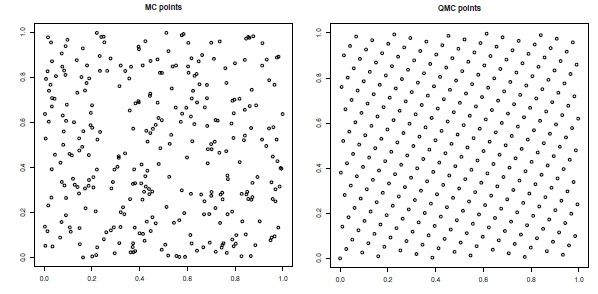
\includegraphics[width=\linewidth]{figs/QMC.jpg}
	\caption{Comparison of MC and QMC sample points\citep{genz2009computation}}
	\label{fig:QMC}
\end{figure}
\end{frame}

\begin{frame}{Quasi Monte Carlo Method}
\footnotesize
\begin{align}
\boldsymbol{\Phi}_n(\mathbf{a}\leq\mathbf{x}\leq\mathbf{b};\boldsymbol{\Sigma})
&=\boldsymbol{\Phi}_n(a\leq\mathbf{Ly}\leq\mathbf{b};I_n)\nonumber\\
&=\int_{a_1\leq l_{11}y_1\leq b_1}\phi(y_1)\cdots\int_{a_n\leq\mathbf{l}_n^t\mathbf{y}\leq b_n}\phi(y_n)d\mathbf{y}\nonumber\\
&=\int_{\tilde{a}_1}^{\tilde{b}_1}\phi(y_1)
\int_{\tilde{a}_2(y_1)}^{\tilde{b}_2(y_1)}\phi(y_2)\cdots
\int_{\tilde{a}_n(y_1,\cdots,y_{n-1})}^{\tilde{b}_n(y_1,\cdots,y_{n-1})}\phi(y_n)d\mathbf{y}\nonumber\\
\text{with } & \tilde{a}_i(y_1,\cdots,y_{i-1})=\frac{a_i-\sum_{j=1}^{i-1}l_{ij}y_j}{l_{ii}}\nonumber\\\text{ and }
&(\tilde{b}_i(y_1,\cdots,y_{i-1}))=\frac{b_i-\sum_{j=1}^{i-1}l_{ij}y_j}{l_{ii}}\nonumber\\
&=\int_{\Phi(\tilde{a}_1)}^{\Phi(\tilde{b}_1)}
\int_{\Phi(\tilde{a}_2(\Phi^{-1}(z_1)))}^{\Phi(\tilde{b}_2(\Phi^{-1}(z_1)))}\cdots
\int_{\Phi(\tilde{a}_n(\Phi^{-1}(z_1),\cdots,\Phi^{-1}(z_{n-1})))}^{\Phi(\tilde{b}_n(\Phi^{-1}(z_1),\cdots,\Phi^{-1}(z_{n-1})))}
d\mathbf{z}(y_i=\Phi^{-1}(z_i))\nonumber\nonumber\\
&=(e_1-d_1)\int_0^1(e_2(w_1)-d_2(w_1))\cdots\nonumber\\
&\int_0^1(e_n(w_1,\cdots,w_{n-1}) - d_n(w_1,\cdots,w_{n-1})))\int_0^1d\mathbf{w}\nonumber\\
\text{with } & z_i=d_i+(e_i-d_i)w_i 
\label{eqn:qmc}
\end{align}
\end{frame}

\begin{frame}{Quasi Monte Carlo Method}
\begin{algorithm}[H]
	\caption{Multivariate Normal Probability with Quasi Monte Carlo Method}
	\begin{algorithmic}[1]
		\tiny
		\Procedure{\texttt{MVN}}{$\boldsymbol{\mu}, \boldsymbol{\Sigma}, \mathbf{a}, \mathbf{b}, ns, N$}
		\State $\mathbf{L}=\text{cholesky}(\boldsymbol{\Sigma})$
		\State $\mathbf{a}=\mathbf{a}-\boldsymbol{\mu}$; $\mathbf{b}=\mathbf{b}-\boldsymbol{\mu}$
		\State $T=0,N=0,V=0$
		\State $\mathbf{p}$ = vector of primes less than $\frac{5n\log{n+1}}{4}$;$\mathbf{q}=\sqrt{\mathbf{p}}$
		\State $\mathbf{P}=\mathbf{1}_{ns}$
		\State $ans = 0$
		\For{$i=1,\cdots,ns$}
		\State $I_i=0$, $\boldsymbol{\Delta}\sim U(0,1)^n$
		\For{$j=1,\cdots,N$}
		\State $\mathbf{X}[1:n,j]=(j+1)\mathbf{q}+\boldsymbol{\Delta}$
		\State $\mathbf{X}[1:n,j]=2\lvert\mathbf{X}[1:n,j]-\text{floor}(\mathbf{X}[1:n,j])\rvert-1$
		\EndFor
		\State $\mathbf{sample}=\mathbf{O}_{n,N}$
		\State $\mathbf{s},\mathbf{c},\mathbf{d},\mathbf{dc}, \mathbf{P}=\mathbf{0}_N$
		\For{$j=1, \cdots,n$}
		\If{$j>1$}
		\State $c=\min(1, c + X[j-1,:]\odot dc)$
		\State $\mathbf{sample}[i-1,1:N] = \Phi^{-1}(c)$
		\State $s = \mathbf{sample}[1:i-1,1:N]^TL[1:i-1, i]$
		\EndIf
		\State $\mathbf{P} *= \Phi(\frac{b-s}{L[i,i]}) - \Phi(\frac{a-s}{L[i,i]})$
		\EndFor
		\State $\text{ans} += \text{mean}(\mathbf{P})$
		\EndFor
		\State\Return $\text{ans}/ns$
		\EndProcedure
	\end{algorithmic}\label{alg:QMC}
\end{algorithm}
\end{frame}

\begin{frame}{Conditioning Approximation}
\footnotesize
\citet{mendell1974multifactorial}, \citet{kamakura1989estimation}, and \citet{trinh2015bivariate} exploit Cholesky factors from LDL decomposition rather than dealing with original covariance matrix.
Biviarate example is follow.
$$\boldsymbol{\Sigma} = \begin{pmatrix}
\boldsymbol{\Sigma}_{1,1} & \mathbf{R}^T\\
\mathbf{R} & \hat{\boldsymbol{\Sigma}}
\end{pmatrix}\text{, with } \mathbf{L}=\begin{pmatrix}
\mathbf{I}_{2} & \mathbf{O}\\1:
\mathbf{M} & \mathbf{L}
\end{pmatrix}\text{ and } \mathbf{D}=\begin{pmatrix}
\mathbf{D}_{1} & \mathbf{O}\\
\mathbf{O} & \mathbf{\hat{D}}
\end{pmatrix}$$
,where $\boldsymbol{\Sigma}_{1,1}, \mathbf{D}_{1}$ is a $2\times2$ matrix. From $\mathbf{D}_1=\boldsymbol{\Sigma_{1,1}}$, $\mathbf{M}=\mathbf{R}\mathbf{D}_1^{-1}$, $\mathbf{\hat{D}}=\hat{\boldsymbol{\Sigma}}-\mathbf{M}\mathbf{D}_1\mathbf{M}^T$
\begin{align}\label{eqn:phi_cond-biv}
\boldsymbol{\Phi}_n(\mathbf{a},\mathbf{b};\mathbf{0},\boldsymbol{\Sigma})
&= \frac{1}{\sqrt{\lvert\mathbf{D}\rvert(2\pi)^n}}\int_{\alpha_1}^{\beta_1}\int_{\alpha_2}^{\beta_2}e^{-\frac{1}{2}\mathbf{x_2}^T\mathbf{D}_1^{-1}\mathbf{x}_2}\nonumber\\
&\cdots \int_{\alpha_{2k-1}}^{\beta_{2k-1}}\int_{\alpha_{2k}}^{\beta_{2k}}e^{-\frac{1}{2}\mathbf{x_{2k}}^T\mathbf{D}_1^{-1}\mathbf{x}_{2k}}
\end{align}
\end{frame}

\begin{frame}{Conditioning Approximation}
\citet{cao2019hierarchical} generalizes bivariate method of \citet{trinh2015bivariate} to $d$-dimensional. Algorithms and details are following.
\begin{algorithm}[H]
	\caption{LDL decomposition}
	\begin{algorithmic}[1]
		\tiny
		\Procedure{\texttt{LDL}}{$\boldsymbol{\Sigma}$}
		\State $\mathbf{L} \leftarrow \mathbf{I}_m, \mathbf{D} \leftarrow \mathbf{O}_m$
		\For{$i = 1:d:m-d+1$}
		\State $\mathbf{D}[i:i+d-1,i:i+d-1] \leftarrow \boldsymbol{\Sigma}[i:i+d-1,i:i+d-1]$
		\State $\mathbf{L}[i+d:m,i:i+d-1] \leftarrow \boldsymbol{\Sigma}[i+d:m,i:i+d-1]\mathbf{D}^{-1}[i:i+d-1,i:i+d-1]$
		\State $\boldsymbol{\Sigma}[i+d:m,i+d:m]\leftarrow\boldsymbol{\Sigma}[i+d:m,i+d:m]-\mathbf{L}[i+d:m,i:i+d-1] \mathbf{D}^{-1}[i:i+d-1,i:i+d-1] \mathbf{L}[i:i+d-1,i+d:m]$
		\If{$i+d<m$}
		\State $\mathbf{D}[i+d:m,i+d:m] \leftarrow \boldsymbol{\Sigma}[i+d:m,i+d:m]$
		\EndIf
		\EndFor
		\State\Return $\mathbf{L}$ and $\mathbf{D}$
		\EndProcedure
	\end{algorithmic}\label{alg:LDL-d}
\end{algorithm}
\end{frame}

\begin{frame}{Conditioning Approximation}
\footnotesize
When $s=\frac{m}{d}$ is integer, results of Algorithm \ref{alg:LDL-d}, $\mathbf{L}, \mathbf{D}$ can be written as
$$
\mathbf{L} = \begin{pmatrix}
\mathbf{I}_d & \mathbf{O}_d & \cdots &\mathbf{O}_d\\
\mathbf{L}_{2,1} & \ddots & \ddots &\vdots\\
\vdots & \ddots & \mathbf{I}_d & \mathbf{O}_d\\
\mathbf{L}_{s,1} & \cdots & \mathbf{L}_{s,s-1} &\mathbf{I}_d\\
\end{pmatrix},
\mathbf{D} = \begin{pmatrix}
\mathbf{D}_1 & \mathbf{O}_d & \cdots &\mathbf{O}_d\\
\mathbf{O}_{d} & \ddots & \ddots &\vdots\\
\vdots & \ddots & \mathbf{D}_{s-1} & \mathbf{O}_d\\
\mathbf{O}_d & \cdots & \mathbf{O}_d &\mathbf{D}_s\\
\end{pmatrix}
$$
with $d$-dimensional identitiy matrix $\mathbf{I}_d$ and $d$-dimensional zero matrix $\mathbf{O}_d$ and $d$-dimensional positive-definite matrix $\mathbf{D}_1,\cdots,\mathbf{D}_s$. 
As in \eqref{eqn:phi_cond-biv}, tranformation, $Y=LX$ provides $m$-dimensional multivariate normal prabability as the product of s $d$-dimensional multivariate normal probabilities as below.
\begin{equation}\label{eqn::phi_cond-ddim}
\boldsymbol{\Phi_m}(\mathbf{a},\mathbf{b};\mathbf{0},\boldsymbol{\Sigma})=\int_{\mathbf{\alpha}_1}^{\mathbf{\beta}_1}\phi_d(\mathbf{y}_1;\mathbf{D}_1)\int_{\mathbf{\alpha}_2}^{\mathbf{\beta}_2}\phi_d(\mathbf{y}_2;\mathbf{D}_2)\cdots\int_{\mathbf{\alpha}_s}^{\mathbf{\beta}_s}\phi_d(\mathbf{y}_s;\mathbf{D}_s)d\mathbf{y}_s\cdots d\mathbf{y}_2d\mathbf{y}_1
\end{equation}
,where $\boldsymbol{\alpha}_i=\mathbf{a}_i-\sum_{j=1}^{i-1}\mathbf{L}_{ij}\mathbf{y}_j, \boldsymbol{\beta}_i=\mathbf{b}_i-\sum_{j=1}^{i-1}\mathbf{L}_{ij}\mathbf{y}_j$
\end{frame}

\begin{frame}{Conditioning Approximation}
\begin{algorithm}[H]
	\caption{d-dimensional conditioning algorithm}
	\begin{algorithmic}[1]
		\footnotesize
		\Procedure{\texttt{CMVN}}{$\boldsymbol{\Sigma},\mathbf{a},\mathbf{b},d$}
		\State $\mathbf{y}\leftarrow\mathbf{0},P\leftarrow1$
		\For{$i = 1:s$}
		\State $j\leftarrow(i-1)d$
		\State $\mathbf{g}\leftarrow\mathbf{L}[j+1:j+d,1:j]\mathbf{y}[1:j]$
		\State $\boldsymbol{\alpha}\leftarrow\mathbf{a}[j+1:j+d]-\mathbf{g}$
		\State $\boldsymbol{\beta}\leftarrow\mathbf{b}[j+1:j+d]-\mathbf{g}$
		\State $\mathbf{D}^\prime\leftarrow\mathbf{D}[j+1:j+d,j+1:j+d]$
		\State $P\leftarrow P\cdot\boldsymbol{\Phi}_d(\boldsymbol{\alpha},\boldsymbol{\beta};\mathbf{0},\mathbf{D}^\prime)$
		\State $\mathbf{y}[j+1:j+d]\leftarrow E[\mathbf{Y}^\prime]$
		\EndFor
		\State\Return $P$ and $\mathbf{y}$
		\EndProcedure
	\end{algorithmic}\label{alg:CMVN}
\end{algorithm}
\end{frame}

\begin{frame}{Multidimensional Truncated Expectations}
\footnotesize
The truncated expectation is expressed as
$$E(X^{e_j})=\frac{1}{\boldsymbol{\Phi}(\mathbf{a},\mathbf{b};\boldsymbol{\mu},\boldsymbol{\Sigma})}\int_\mathbf{a}^\mathbf{b}x_j\phi_d(\mathbf{x};\boldsymbol{\mu},\boldsymbol{\Sigma})d\mathbf{x}=\frac{1}{\boldsymbol{\Phi}(\mathbf{a},\mathbf{b};\boldsymbol{\mu},\boldsymbol{\Sigma})}F_j^d(\mathbf{a},\mathbf{b};\boldsymbol{\mu},\boldsymbol{\Sigma})$$

\begin{theorem}\citep{kan2017moments}
	\label{thm:thmkan}
	$$F_j^d(\mathbf{a},\mathbf{b};\boldsymbol{\mu},\boldsymbol{\Sigma})= \mu_j\boldsymbol{\Phi}_d(\mathbf{a},\mathbf{b};\boldsymbol{\mu},\boldsymbol{\Sigma})+\mathbf{e}_j^T\boldsymbol{\Sigma}\mathbf{c}$$
	,where $c$ is a vector with lth component defined as
	$$\begin{aligned}
	c_l&=\phi_1(a_l;\mu_l,\sigma_l^2)\Phi_{d-1}(\mathbf{a}_{-l},\mathbf{b}_{-l};\boldsymbol{\hat{\mu}}^1, \hat{\boldsymbol{\Sigma}}_l)
	-\phi_1(b_l;\mu_l,\sigma_l^2)\Phi_{d-1}(\mathbf{a}_{-l},\mathbf{b}_{-l};\boldsymbol{\hat{\mu}}^2, \hat{\boldsymbol{\Sigma}}_l)\\
	\boldsymbol{\hat{\mu}}^1_l&=\mu_{-l}+\boldsymbol{\Sigma}_{-l,l}\frac{a_l-\mu_l}{\sigma_l^2},
	\boldsymbol{\hat{\mu}}^2_l=\mu_{-l}+\boldsymbol{\Sigma}_{-l,l}\frac{b_l-\mu_l}{\sigma_l^2},\\
	\hat{\boldsymbol{\Sigma}}_l&=\boldsymbol{\Sigma}_{-l,-l} -\frac{1}{\sigma_l^2}\boldsymbol{\Sigma}_{-l,l}\boldsymbol{\Sigma}_{l,-l}
	\end{aligned}$$
\end{theorem}
Theorem \ref{thm:thmkan} has same form with bivariate version of \citet{trinh2015bivariate} with $d=2$ and it allows us to calculate $E[Y^\prime]$ in Algorithm \ref{alg:CMVN} with $\boldsymbol{\Phi}$ which can be obtained with quasi monte calro method proposed by \citet{genz1992numerical}
\end{frame}

\begin{frame}{Multidimensional Conditioning Approximation with Univariate Reordering}
\footnotesize
Appropriate integration order on conditioning algorithm possibly improves estiation accuracy
\begin{itemize}
	\item \citet{schervish1984algorithm} : integral with shortest integration interval widths be the outermost integration variables
	\item \citet{gibson1994monte} : variables which have smallest expected values be the outermost integration variables.\\
	Since innermost integrals which have smaller variation have the most influence with this order, overall variance reduces.
	\item \citet{trinh2015bivariate} also employs this ordering, and \citet{cao2019hierarchical} generalized it to $d$-dimensional problem.
\end{itemize}
\end{frame}

\begin{frame}{Multidimensional Conditioning Approximation with Univariate Reordering}
\begin{algorithm}[H]
	\caption{d-dimensional conditioning algorithm with univariate reordering}
	\begin{algorithmic}[1]
		\tiny
		\Procedure{\texttt{RCMVN}}{$\boldsymbol{\Sigma},\mathbf{a},\mathbf{b},d$}
		\State $\mathbf{y}\leftarrow\mathbf{0},\mathbf{C}\leftarrow\boldsymbol{\Sigma}$
		\For{$i = 1:m$}
		\If{$i > 1$}
		\State $\mathbf{y}[i-1]\leftarrow\frac{\phi(a^\prime)-\phi(b^\prime)}{\Phi(b^\prime)-\Phi(a^\prime)}$
		\EndIf
		\State $j\leftarrow\text{argmin}_{i\leq j\leq m}\{\Phi(\frac{\mathbf{b}[j]-\mathbf{C}[j,1:i-1]\mathbf{y}[1:i-1]}{\sqrt{\boldsymbol{\Sigma}[j,j]-\mathbf{C}[j,1:i-1]\mathbf{C}^T[j,1:i-1]}})-\Phi(\frac{\mathbf{a}[j]-\mathbf{C}[j,1:i-1]\mathbf{y}[1:i-1]}{\sqrt{\boldsymbol{\Sigma}[j,j]-\mathbf{C}[j,1:i-1]\mathbf{C}^T[j,1:i-1]}})\}$
		\State $\boldsymbol{\Sigma}[:,(i,j)]\leftarrow\boldsymbol{\Sigma}[:,(j,i)]$;$\boldsymbol{\Sigma}[(i,j),:]\leftarrow\boldsymbol{\Sigma}[(j,i),:]$
		\State $\mathbf{C}[:,(i,j)]\leftarrow\mathbf{C}[:,(j,i)]$;$\mathbf{C}[(i,j),:]\leftarrow\mathbf{C}[(j,i),:]$
		\State $\mathbf{a}[(i,j)]=\mathbf{a}[(j,i)]$
		\State $\mathbf{b}[(i,j)]=\mathbf{b}[(j,i)]$
		\State $\mathbf{C}[i,i]\leftarrow\sqrt{\boldsymbol{\Sigma}[i,i]-\mathbf{C}[i,1:i-1]\mathbf{C}^T[i,1:i-1]}$
		\State $\mathbf{C}[j,i]\leftarrow \frac{\boldsymbol{\Sigma}[j,i]-\mathbf{C}[i,1:i-1]\mathbf{C}^T[j,1:i-1]}{\mathbf{C}[i,i]}$, for $j=i+1,\cdots,m$
		\State $a^\prime=\frac{\mathbf{a}[i]-\mathbf{C}[i,1:i-1]y[1:i-1]}{\mathbf{C[i,i]}}$
		\State $b^\prime=\frac{\mathbf{b}[i]-\mathbf{C}[i,1:i-1]y[1:i-1]}{\mathbf{C[i,i]}}$
		\EndFor
		\State\Return \texttt{CMVN}($\boldsymbol{\Sigma},\mathbf{a},\mathbf{b},d$) as in Algorithm \ref{alg:CMVN}
		\EndProcedure
	\end{algorithmic}\label{alg:RCMVN}
\end{algorithm}

\end{frame}
\section{Hierarchical-Block Approximation}

\begin{frame}{Hierarchical Cholesky Decomposition}
\footnotesize
\citet{hackbusch2015hierarchical} proposed hiarchical matrix and its cholesky decomposition method.
$A=LU$ have the structure
$$\begin{pmatrix}A_{11}&A_{12}\\A_{21}&A_{22}\end{pmatrix}=\begin{pmatrix}L_{11}&O\\L_{21}&L_{22}\end{pmatrix}\begin{pmatrix}L_{11}^T&L_{12}^T\\O&L_{22}^T\end{pmatrix}$$
with lower triangular matrix $L_{11},L_{22}$.
It leads to four tasks:
\begin{itemize}
	\item[(a)] compute $L_{11}$ via Cholesky decomposition of $A_{11}$
	\item[(b)] compute $L_{12}$ from $L_{21}L_{11}^T = A_{21}$
	\item[(c)] low rank approximation of $L_{12}=UV^T$
	\item[(d)] compute $L_{22}$ via Cholesky decomposition of $A_{22}-L_{21}L_{21}^T$
\end{itemize}

We have applied low rank approximation with svd to (c) each block of its decomposition to make implementation efficiently and save storage while accuracy is preserved.
: i.e. $A=UDV^T=\sum_{i=1}^n d_i u_iv_i^T\approx\sum_{i=1}^k d_i u_iv_i^T$.
\end{frame}

\begin{frame}{Hierarchical Cholesky Decomposition}
Hierachical cholesky decomposition of $n\times n$ matrix into $m\times m$ blocks is implemented like below.
\begin{algorithm}[H]
	\caption{Hierachical cholesky decomposition}
	\begin{algorithmic}[1]
		\tiny
		\Procedure{\texttt{hchol}}{$A$, n,m,rank}
		\For{$i=1:log_2(\frac{n}{m})$}
		\State $nb = n/2^i$
		\State x = 0, y = nb
		\For{$j=1:2^{i-1}$}
		\State $\mathbf{U,D,V} = lowrankSVD(A[xbegin+1:xbegin+nb,ybegin+1:ybegin+nb], rank)$
		\State $\mathbf{A}[x + 1:x + nb, y + 1:y + rank] = \mathbf{UD}$
		\State $\mathbf{A}[x + 1:x + nb, y + rank+1:y + nb] = \mathbf{O}$
		\State $\mathbf{A}[y + 1:y + nb, x + 1:x + rank] = \mathbf{VD}$
		\State $\mathbf{A}[y + 1:y + nb, x + rank+1:x + nb] = \mathbf{O}$
		\State $x += 2nb, y += 2nb$
		\EndFor
		\EndFor
		\EndProcedure
		
	\end{algorithmic}\label{alg:hchol}
\end{algorithm}
\end{frame}

\begin{frame}{The Hierarchical-Block Conditioning Method}
\footnotesize
Let $\phi_m(\mathbf{x}; \boldsymbol{\Sigma})$ be a pdf of the $m$-dimensional normal distribution $N(\mathbf{0}, \boldsymbol{\Sigma})$ and $(\mathbf{B}, \mathbf{U}\mathbf{V}^T)$ be the hierarchical Cholesky decompostion of the covariance matrix $\boldsymbol{\Sigma}$. Then,
\begin{equation}\label{eqn:hmvn}
\Phi_n(\mathbf{a}, \mathbf{b}; \mathbf{0}, \boldsymbol{\Sigma}) 
= \int_{\mathbf{a}_1'}^{\mathbf{b}_1'} \phi_m(\mathbf{x}_1; \mathbf{B}_1\mathbf{B}_1^T) 
\cdots 
\int_{\mathbf{a}_r'}^{\mathbf{b}_r'} \phi_r(\mathbf{x}_r; \mathbf{B}_r\mathbf{B}_r^T) d\mathbf{x}_r \cdots d\mathbf{x}_1.
\end{equation}
,where $\mathbf{a}',~\mathbf{b}'$, $i=1,\cdots,r$, are the corresponding segments of the updated $\mathbf{a}$ and $\mathbf{b}$. 

Note the probabilities $\Phi_m(\mathbf{a}_i, \mathbf{b}_i; \mathbf{0}, \mathbf{B}_i\mathbf{B}_i^T)$ can be computed using
\begin{itemize}
	\item[1.] Quasi-Monte Carlo method (\texttt{HMVN}, Method 1 in \citet{cao2019hierarchical})
	\item[2.] $d$-dimensional conditioning algorithm (\texttt{HCMVN}, Method 2 in \citet{cao2019hierarchical})
	\item[3.] $d$-dimensional conditioning algorithm with univariate reordering (\texttt{HRCMVN}, Method 3 in \citet{cao2019hierarchical}). 
\end{itemize} 
These methods are more effective and easily parallelizable than the classical methods.
\end{frame}

\begin{frame}{The Hierarchical-Block Conditioning Method}
\begin{algorithm}[H]
	\caption{Hierarchical-block conditioning algorithm}
	\begin{algorithmic}[1]
		\tiny
		\Procedure{\texttt{HMVN}}{$a,~b,~\boldsymbol{\Sigma},~d$}
		\State $\mathbf{x} \leftarrow \mathbf{0}$ and $P \leftarrow 1$
		\State $[\mathbf{B}, \mathbf{UV}] \leftarrow$ \texttt{choldecomp\_hmatrix}$(\boldsymbol{\Sigma})$
		\For{$i = 1:r$}
		\State $j \leftarrow (i-1)m$
		\If{$i>1$}
		\State $o_r \leftarrow$ row offset of $\mathbf{U}_{i-1}\mathbf{V}_{i-1}^T$
		\State $o_c \leftarrow$ column offset of $\mathbf{U}_{i-1}\mathbf{V}_{i-1}^T$
		\State $l \leftarrow \dim(\mathbf{U}_{i-1}\mathbf{V}_{i-1}^T)$
		\State $\mathbf{g} \leftarrow \mathbf{U}_{i-1}\mathbf{V}_{i-1}^T\mathbf{x}[o_c+1:o_c+l]$
		\State $\mathbf{a}[o_r+1:o_r+l] = \mathbf{a}[o_r+1:o_r+l] - \mathbf{g}$
		\State $\mathbf{b}[o_r+1:o_r+l] = \mathbf{a}[o_r+1:o_r+l] - \mathbf{g}$
		\EndIf
		\State $\mathbf{a}_i \leftarrow \mathbf{a}[j+1:j+m]$
		\State $\mathbf{b}_i \leftarrow \mathbf{b}[j+1:j+m]$
		\State $P = P*\Phi_m(\mathbf{a}_i, \mathbf{b}_i; \mathbf{0}, \mathbf{B}_i\mathbf{B}_i^T)$
		\State $\mathbf{x}[j+1:j+m] \leftarrow \mathbf{B}_{i}^{-1} E(\mathbf{X}_i)$
		\EndFor
		\EndProcedure
	\end{algorithmic}\label{alg:hmvn}
\end{algorithm}
\end{frame}

\begin{frame}{Computational Complexity}
\footnotesize

$M(\cdot)$ denotes the complexity of the QMC simulation in the given dimension. \\
Table \ref{tbl:cc_hmvn} shows that the time efficiency of the $d$-dimensional conditioning algorithm mainly comes from lowering the dimension in which the QMC simulation is performed. 
\renewcommand{\arraystretch}{1.5}
\begin{table}[ht]
	\begin{center}
		\begin{tabular}{l l l l}
			& MVN prob                     & Trunc exp          & Upd limits            \\
			\hline
			\texttt{HMVN}   & $\frac{n}{m} M(m)$           & $2nM(m) + O(nm^2)$ & $O(mn + kn log(n/m))$ \\
			\texttt{HCMVN}  & $\frac{n}{d} M(d) + O(m^2n)$ & $2nM(d) + O(nd^2)$ & $O(mn + kn log(n/m))$ \\
			\texttt{HRCMVN} & $\frac{n}{d} M(d) + O(m^2n)$ & $2nM(d) + O(nd^2)$ & $O(mn + kn log(n/m))$ \\
			\hline
		\end{tabular}
		\caption{Complexity decomposition of the \texttt{HMVN}, \texttt{HCMVN}, and \texttt{HRCMVN}}\label{tbl:cc_hmvn}
	\end{center}
\end{table}
\renewcommand{\arraystretch}{1}

\begin{itemize}
	\item The updating cost is independent of the method.
	\item The complexity of the univariate reordering is $O(m^2 n)$, the same as the complexity of computing the MVN probabilities in \texttt{HCMVN}
	\item Since \texttt{HCMVN} and \texttt{HRCMVN} perform the QMC  simulation in $d$-dimensions, these two methods are not greatly affected by the choice of $m$.
\end{itemize}
\end{frame}

\section{Block Reordering}

\begin{frame}{Block Reordering}
\footnotesize
\begin{itemize}
	\item The cdf value for $n$-dimensioned multivariate normal variable comprises of $m$ multiplications of $d$-dimensional integrals.
	\item Recall the \texttt{RCMVN} algorithm(\ref{alg:CMVN}) : as computing each $d$-dimensional integral values, integration variables were arranged in order of increasing order of \texttt{CMVN} probability values, from outer to inner
	\item Permutes the block of LDL-decomposed covariance matrix, in order of \texttt{RCMVN} probability values of each blocks
	\item Result accuracy and time cost is compared among \texttt{HMVN}, \texttt{HCMVN}, \texttt{HRCMVN} with/without block reordering.
\end{itemize}
\end{frame}

\begin{frame}{Block Reordering}
\begin{algorithm}[H]
\caption{Blockwise reordering}
\begin{algorithmic}
	\tiny
	\Procedure{\texttt{Blockreorder}}{$G,~\rho,~a,~b,~m,~ind$}
	\State $G, \rho, a, b, m, ind$ given, $\mathbf{P}$ $\leftarrow$ $0$
	\For{$i = 1:m:n-m+1$}
	\State $\mathbf{s}$ $\leftarrow$ $ind[i:i+m-1]$
	\State $\mathbf{A}$ $\leftarrow$ $\rho(G, \mathbf{s})$
	\State $a'$ $\leftarrow$ $a[\mathbf{s}]$
	\State $b'$ $\leftarrow$ $b[\mathbf{s}]$
	\State $\mathbf{P}$ $\leftarrow$ $[\mathbf{P}, \texttt{RCMVN}(\mathbf{A},a',b',1).P]$
	\EndFor
	\State sort(ind, $\mathbf{P}$, m)
	\State \Return ind
	\EndProcedure
\end{algorithmic}\label{alg:BR}	
\end{algorithm}
\end{frame}

\begin{frame}{Block Reordering}
\begin{algorithm}[H]
	\caption{Hierarchical-block conditioning algorithm with Block Reordering}
	\begin{algorithmic}
		\tiny
		\Procedure{\texttt{HCMVN\_BRO}}{$a,~b,~\Sigma,~d$}
		\State $\mathbf{x} \leftarrow \mathbf{0}$, $P \leftarrow 1$, ind $\leftarrow$ $[1,\dots, n]$
		\State $[\mathbf{B}, \mathbf{UV}] \leftarrow$ \texttt{choldecomp\_hmatrix}$(\Sigma)$
		\State $\mathbf{B} \leftarrow$ \texttt{Blockreorder}($G, \rho, a, b, m, ind$)
		\For{$i = 1:r$}
		\State $j \leftarrow (i-1)m$
		\If{$i>1$}
		\State $o_r \leftarrow$ row offset of $\mathbf{U}_{i-1}\mathbf{V}_{i-1}^T$
		\State $o_c \leftarrow$ column offset of $\mathbf{U}_{i-1}\mathbf{V}_{i-1}^T$
		\State $l \leftarrow \dim(\mathbf{U}_{i-1}\mathbf{V}_{i-1}^T)$
		\State $\mathbf{g} \leftarrow \mathbf{U}_{i-1}\mathbf{V}_{i-1}^T\mathbf{x}[o_c+1:o_c+l]$
		\State $\mathbf{a}[o_r+1:o_r+l] = \mathbf{a}[o_r+1:o_r+l] - \mathbf{g}$
		\State $\mathbf{b}[o_r+1:o_r+l] = \mathbf{a}[o_r+1:o_r+l] - \mathbf{g}$
		\EndIf
		\State $\mathbf{a}_i \leftarrow \mathbf{a}[j+1:j+m]$
		\State $\mathbf{b}_i \leftarrow \mathbf{b}[j+1:j+m]$
		\State $P = P*\Phi_m(\mathbf{a}_i, \mathbf{b}_i; \mathbf{0}, \mathbf{B}_i\mathbf{B}_i^T)$
		\State $\mathbf{x}[j+1:j+m] \leftarrow \mathbf{B}_{i}^{-1} E[\mathbf{X}_i]$
		\EndFor
		\EndProcedure
	\end{algorithmic}\label{alg:hmvn_bro}
\end{algorithm}

\end{frame}
\section{Numerical Examples}

\subsection{Cholesky Factorization}

\begin{frame}{Cholesky Factorization}
	
	\begin{block}{Data}
		Exponential covariance matrix, $\boldsymbol{\Sigma}_{ij}=exp(-\lVert \mathbf{s}_i-\mathbf{s}_j \rVert/\beta)$ is set with $\beta=0.3$. $n$ points, $\mathbf{s}_1,\cdots,\mathbf{s}_n$ is evenly distributed over unique square with Morton's order which defined recursively as described in figure \ref{fig:morton}.
	\end{block}

	\begin{figure}[h]
		\centering
		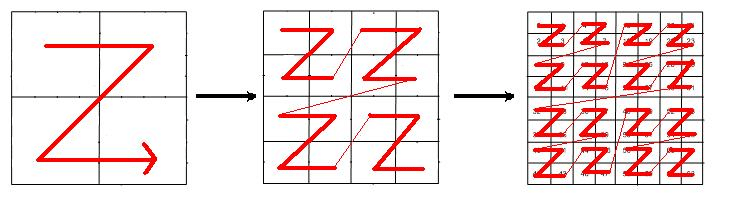
\includegraphics[width=.7\linewidth]{figs/Morton.jpg}
		\caption{Morton's order \citep{salem2016comparative}}
		\label{fig:morton}
	\end{figure}
\end{frame}

\begin{frame}{Cholesky Factorization}
	\begin{block}{Methods}
		\begin{enumerate}
			\item The \textit{chol} function from \textbf{LinearAlgebra} package
			\item The \textit{dpotrf} from \textbf{LAPACK} package
			\item Hierarchical cholesky decomposition which suggested by \citet{hackbusch2015hierarchical} are implemented. 
		\end{enumerate}
	\end{block}
	
	\begin{itemize}
		\item With various $n$, three Cholesky methods are applied and results are below table \ref{tab:table1}. 
		\item In low rank approximation at algorithm \ref{alg:hchol}, rank is about $n^{1/4}$.
		\item Hierarchical cholesky decomposition provides $\boldsymbol{\Sigma}\approx L_HL_H^T$. 
		\item Its relative error is defined as 
		$\dfrac{\lVert\boldsymbol{\Sigma}-L_HL_H^T\rVert_2}{\lVert\boldsymbol{\Sigma}\rVert_2}$
	\end{itemize}
	
\end{frame}

\begin{frame}{Cholesky Factorization}

\begin{table}[h]
	\centering
	\resizebox{.8\textwidth}{!}{
		\begin{tabular}{@{}ccccc@{}}
			\toprule
			n & 256 & 1024 & 4096 & 16384 \\ \midrule
			chol & 0.001s & 0.0097s & 0.414s & 156.3s \\
			dpotrf & 0.0007s & 0.0132s & 0.431s & 154.1s \\
			hierarchical cholesky & 0.153s & 0.076s & 0.916s & 37.3s \\
			Error of hierarchical cholesky & 1.06e-7 & 9.97e-7 & 1.11e-3 & 1.87e-3 \\  \bottomrule
		\end{tabular}%
	}
	\caption{Excution times for Cholesky factorization}
	\label{tab:table1}
\end{table}

\begin{block}{Results}
	\begin{itemize}
		\item Hierarchical cholesky decomposition is more efficient than other classical cholesky method with large dimension.
		\item Table \ref{tab:table1} ensures accuracy of hierarchical cholesky decomposition proposed by \citet{hackbusch2015hierarchical}.
	\end{itemize}
\end{block}

\end{frame}

\subsection{Multidimensional Conditioning Approximations}

\begin{frame}{Multivariate Normal Probabilities} 

	\begin{block}{Methods}
		\begin{enumerate}
			\item Classical Monte Carlo(MC) is estimate probabilities from acceptance ratio
			\item Richtmyer Quasi-Monte Carlo(QMC) introduced in subsection \ref{subsec:qmc}
		\end{enumerate}
	\end{block}

	\begin{block}{Settings}
		\begin{itemize}
			% \item We implement \texttt{mvn}, the function that calculate multivariate normal probabilities using Richtmyer QMC method introduced in subsection \ref{subsec:qmc}. 
			\item Varying sample size $N$ and dimension $d$, two Monte Carlo methods are compared and results are below table \ref{tab:results_mc} and \ref{tab:results_qmc}. 
			\item Set $\Sigma = I_d$, $\mathbf{a}_i = -\infty$ and $\mathbf{b}_i = 0$, i.e. true probabilities are $1/2^d$s
			\item Repeat 20 times.
			% \item All the multivariate normal distribution probabilities required in the next algorithms are calculated using the \texttt{mvn} function.
		\end{itemize}
	\end{block}

\end{frame}
	
\begin{frame}{Multivariate Normal Probabilities} 
	
	\begin{table}[!h]
		\centering
		% \resizebox{.6\textwidth}{!}{%
		{
			\begin{tabular}{@{}cccccc@{}}
				\toprule
				$(n, d)$ 				  & 4 		& 8 	  & 12 		& 16 	  & 20	 \\ \midrule
				\multirow{2}{*}{500}  & 12.2\%  & 56.8\%  & 161.9\% & 100.0\% & 100.0\% \\
									  & 0.294ms & 0.016ms & 0.018ms & 0.019ms & 0.019ms \\
				\multirow{2}{*}{1000} & 9.5\%   & 50.6\%  & 193.8\% & 100.0\% & 100.0\% \\
									  & 0.046ms & 0.041ms & 0.028ms & 0.028ms & 0.034ms \\
				\multirow{2}{*}{1500} & 8.9\%   & 38.7\%  & 150.2\% & 100.0\% & 100.0\% \\
									  & 0.055ms & 0.046ms & 0.042ms & 0.048ms & 0.045ms \\
				\multirow{2}{*}{2000} & 5.4\%   & 26.5\%  & 102.4\% & 100.0\% & 100.0\% \\
									  & 0.070ms & 0.065ms & 0.072ms & 0.058ms & 0.055ms \\
				\multirow{2}{*}{2500} & 5.1\%   & 32.0\%  & 100.1\% & 100.0\% & 100.0\% \\
									  & 0.073ms & 0.092ms & 0.081ms & 0.083ms & 0.076ms \\
				\bottomrule
			\end{tabular}%
		}
		\caption{Results for the classical Monte Carlo}
		\label{tab:results_mc}
	\end{table}	

\end{frame}

\begin{frame}{Multivariate Normal Probabilities} 
	\begin{table}[!h]
		\centering
		% \resizebox{.6\textwidth}{!}{%
		{
			\begin{tabular}{@{}cccccc@{}}
				\toprule
				$(n, d)$ 				  & 4 		& 8 	  & 12 		& 16 	  & 20	 \\ \midrule
				\multirow{2}{*}{500}  & 0.0\%   & 0.0\%   & 0.0\%   & 0.0\%   & 0.0\% \\
									& 0.058ms & 0.003ms & 0.006ms & 0.006ms & 0.011ms \\
				\multirow{2}{*}{1000} & 0.0\%   & 0.0\%   & 0.0\%   & 0.0\%   & 0.0\% \\
									& 0.003ms & 0.009ms & 0.013ms & 0.017ms & 0.020ms \\
				\multirow{2}{*}{1500} & 0.0\%   & 0.0\%   & 0.0\%   & 0.0\%   & 0.0\% \\
									& 0.006ms & 0.011ms & 0.016ms & 0.019ms & 0.030ms \\
				\multirow{2}{*}{2000} & 0.0\%   & 0.0\%   & 0.0\%   & 0.0\%   & 0.0\% \\
									& 0.011ms & 0.012ms & 0.013ms & 0.025ms & 0.036ms \\
				\multirow{2}{*}{2500} & 0.0\%   & 0.0\%   & 0.0\%   & 0.0\%   & 0.0\% \\
									& 0.009ms & 0.022ms & 0.033ms & 0.038ms & 0.056ms \\ \bottomrule
			\end{tabular}%
		}
		\caption{Results for the Richtmyer Quasi-Monte Carlo}
		\label{tab:results_qmc}
	\end{table}

\end{frame}

\begin{frame}{\subsecname}
	\begin{block}{Results}
		\begin{itemize}
			% \item QMC is superior to MC in every criterion.
			\item MC fails even $d$ is not large enough. 
			\item QMC is numerically stable and faster than MC 
			\item All the multivariate normal distribution probabilities required in the next experiments are calculated using QMC.
		\end{itemize}
		% \begin{itemize}
			% \item To summarize the results, QMC is superior to MC in every criterion. 
			% \item All the multivariate normal distribution probabilities required in the next algorithms are calculated using the \texttt{mvn} function.
		% \end{itemize}
	\end{block}
\end{frame}

\begin{frame}{d-dimensional Conditioning Algorithm without/with Reordering}

	% \footnotesize

\begin{block}{Settings}
	\begin{itemize}
		\item 250 MVN problems with various values of $m$ and $d$
		\item $\boldsymbol{\Sigma}=\mathbf{Q}\mathbf{J}\mathbf{Q}^T$ is simulated with $\mathbf{Q}\sim{Haar~distribution}$ and $J=diag(j_i)$ where $j_1,\cdots,j_m\sim U(0,1)$
		\item Integration limits $a_i=-\infty$ and $b_i\sim(U,m)$ for $i=1\cdots,m$
	\end{itemize}
\end{block}

\begin{theorem}\label{thm:haar}\citet{stewart1980efficient}
	Let the independent vectors $x_1,\cdots,x_{n}$ be distributed $N(0,\sigma^2 \mathbf{I})$. For $j=1,2,\cdots,n-1$, let $\mathbf{\bar{H}}_{x_j}$ be the Householder transformation that reduces $x_j$ to $r_{jj}e_1$, where $r_{ij}$ is obtained in QR decomposition of $[x_1,\cdots,x_n]$ Let $\mathbf{H}_j=diag(\mathbf{I}_{j-1},\bar{\mathbf{H}}_j)$. Let $\mathbf{D}=diag(sign(r_{11}), \cdots, sign(r_{nn}))$. Then the product $\mathbf{Q}=\mathbf{DH_1\cdots H_{n-1}}$ follows Haar Distribution.
\end{theorem}

\end{frame}
	
\begin{frame}{d-dimensional Conditioning Algorithm without/with Reordering}
\tiny

\begin{table}[h]
	\centering
	\resizebox{.7\textwidth}{!}{
		\begin{tabular}{@{}cccccc@{}}
			\toprule
			$(m, d)$ & 1 & 2 & 4 & 8 & 16 \\ \midrule
			\multicolumn{6}{l}{Without univariate reordering} \\ \midrule
			\multirow{2}{*}{16} & 3.7\% & 3.5\% & 3.6\% & 3.8\% & 2.9\% \\
			& 0.029ms & 0.201ms & 0.431ms & 0.676ms & 1.372ms \\
			\multirow{2}{*}{32} & 2.4\% & 2.9\% & 2.9\% & 3.3\% & 2.7\% \\
			& 0.001ms & 0.390ms & 0.833ms & 1.283ms & 2.545ms \\
			\multirow{2}{*}{64} & 1.9\% & 2.1\% & 2.1\% & 1.8\% & 1.9\% \\
			& 0.004ms & 0.762ms & 1.686ms & 2.545ms & 5.004ms \\
			\multirow{2}{*}{128} & 1.3\% & 1.5\% & 1.3\% & 1.2\% & 1.4\% \\
			& 0.024ms & 1.505ms & 3.333ms & 5.146ms & 10.548ms \\ \midrule
			\multicolumn{6}{l}{With univariate reordering} \\ \midrule
			\multirow{2}{*}{16} & 3.3\% & 3.1\% & 3.3\% & 3.6\% & 2.7\% \\
			& 0.007ms & 0.203ms & 0.439ms & 0.680ms & 1.363ms \\
			\multirow{2}{*}{32} & 2.3\% & 2.6\% & 2.6\% & 3.2\% & 2.6\% \\
			& 0.004ms & 0.393ms & 0.841ms & 1.289ms & 2.544ms \\
			\multirow{2}{*}{64} & 2.0\% & 2.1\% & 2.1\% & 1.9\% & 1.9\% \\
			& 0.014ms & 0.773ms & 1.695ms & 2.552ms & 5.022ms \\
			\multirow{2}{*}{128} & 1.2\% & 1.5\% & 1.4\% & 1.2\% & 1.4\% \\
			& 0.097ms & 1.593ms & 3.462ms & 5.268ms & 10.7861ms \\ \bottomrule
		\end{tabular}%
	}
	\caption{Errors and execution times of the d-dimensional conditioning method}
	\label{tab:table2}
\end{table}
% \footnotesize
	% 
\end{frame}

\begin{frame}{\subsecname}

	\begin{block}{Results}
		\begin{itemize}
			\item Estimated value is compared with approximated value obtained via quasi monte carlo method with a sample size of $10^4$, which ensures error below $10^{-4}$
			\item Estimation error tended to decrease as $d$ increases with each $m$ since lager $d$ implers less discarded correlation information. 
			\item Spent time grows to a linear fashion with m while it grows exponentially with $d$.
		\end{itemize}
	\end{block}
	
\end{frame}

\subsection{Hierarchical-Block Approximations}

\begin{frame}{\subsecname}

	\begin{block}{Methods}
		\begin{itemize}
			\item M1, \texttt{HMVN()}: Calculate multivariate normal probabilities using hierarchical-block approximation
			\item M2, \texttt{HCMVN()}: Calculate multivariate normal probabilities using hierarchical-block conditioning approximation
			\item M3, \texttt{HRCMVN()}: Calculate multivariate normal probabilities using hierarchical-block conditioning approximation with univarite reordering
		\end{itemize}
	\end{block}

	\begin{block}{Data}
		\begin{enumerate}
			\item Constant covariance matrix: $k(x_i, x_j) = \theta + (1-\theta)\delta_{ij}$ for some $|\theta| < 1$.
			\item 1D exponential covariance matrix: $k(x_i, x_j) = \exp(-d_{ij}/\beta)$ for some $\beta > 0$, where $d_{ij}$ is the distance between $x_i$ and $x_j$.
		\end{enumerate}
	\end{block}

\end{frame}

\begin{frame}{\subsecname}

	\begin{block}{Settings}
		\begin{itemize}
			\item Simulation size = 20
			\item Integration limits $a_i=-\infty$ and $b_i\sim(U,n)$ for $i=1\cdots,n$
			\item $\theta=0.7$, $d_{ij} = 1$, and $\beta=10$ as in \citet{cao2019hierarchical}
			\item Fix $d=4$ for \texttt{HCMVN} and \texttt{HRCMVN}.
		\end{itemize}
	\end{block}

	Table \ref{tab:table3}, Figure \ref{fig:table3_htime} and \ref{fig:table3_hctime} are errors and execution times under the constant covariance structure and 1D exponential covariance structure respectively. 
\end{frame}

\begin{frame}{\subsecname}

	\begin{table}[!h]
		\centering	
		\resizebox{\textwidth}{!}{
			\begin{tabular}{@{}llllllllll@{}}
				\toprule
				$m$ 	& \multicolumn{3}{l}{16} & \multicolumn{3}{l}{32} & \multicolumn{3}{l}{64}  \\
				$n$ 	& 256 & 512 & 1024 & 256 & 512 & 1024 & 256 & 512 & 1024 \\ \bottomrule
				
				\multicolumn{10}{l}{Constant covariance structure} \\ \midrule
	
				M1 & 8.22\% & 7.11\% & 8.66\% & 8.94\% & 7.88\% & 6.68\% & 10.58\% & 8.05\% & 9.78\% \\
				M2 & 8.37\% & 7.08\% & 8.60\% & 8.91\% & 7.77\% & 6.61\% & 10.58\% & 8.26\% & 9.91\% \\
				M3 & 8.51\% & 7.10\% & 8.70\% & 9.51\% & 7.92\% & 7.00\% & 10.68\% & 7.94\% & 9.63\% \\
	
				\midrule
				
				\multicolumn{10}{l}{1D exponential covariance matrix} \\ \midrule
	
				M1 & 2.87\% & 0.00\% & 0.01\% & 0.07\% & 1.31\% & 0.00\% & 2.65\% & 0.27\% & 0.57\% \\
				M2 & 3.28\% & 0.01\% & 0.90\% & 0.07\% & 1.31\% & 0.01\% & 2.65\% & 0.28\% & 0.57\% \\
				M3 & 4.73\% & 0.09\% & 2.11\% & 2.17\% & 1.90\% & 0.16\% & 3.72\% & 1.25\% & 0.66\% \\
					
				\bottomrule
			\end{tabular}%
		}
		\caption{Relative errors under the constant covariance structure and 1D exponential covariance structure}
		\label{tab:table3}
	\end{table}
	
\end{frame}

\begin{frame}[allowframebreaks]{\subsecname - Execution Time}
	\begin{figure}
		\centering
		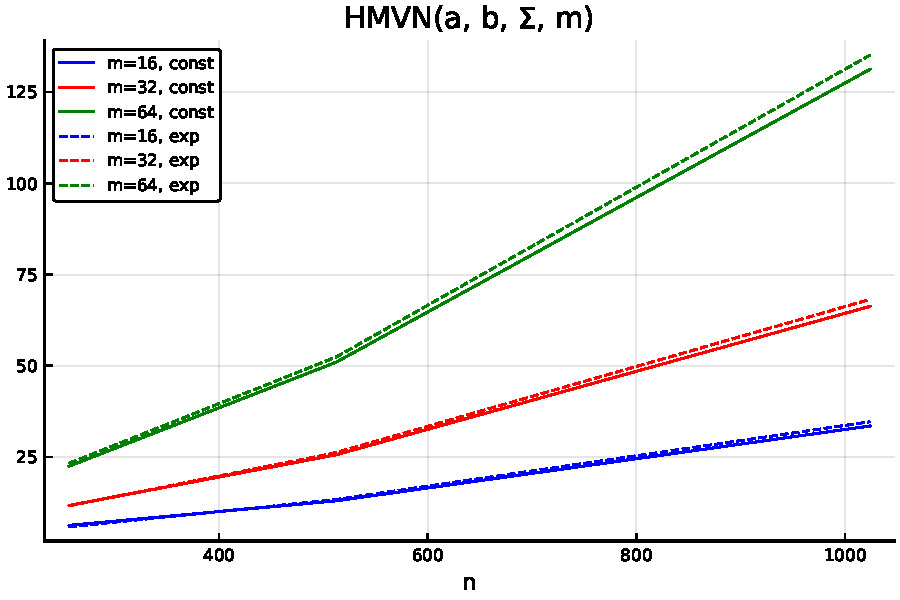
\includegraphics[width=0.8\linewidth]{figs/table3_m1.pdf}
		\caption{Execution time (seconds) for the hierarchical-block approximation}\label{fig:table3_htime}
	\end{figure}

	\framebreak

	\begin{figure}
		\centering
				\begin{subfigure}[b]{0.45\textwidth}
						\centering
						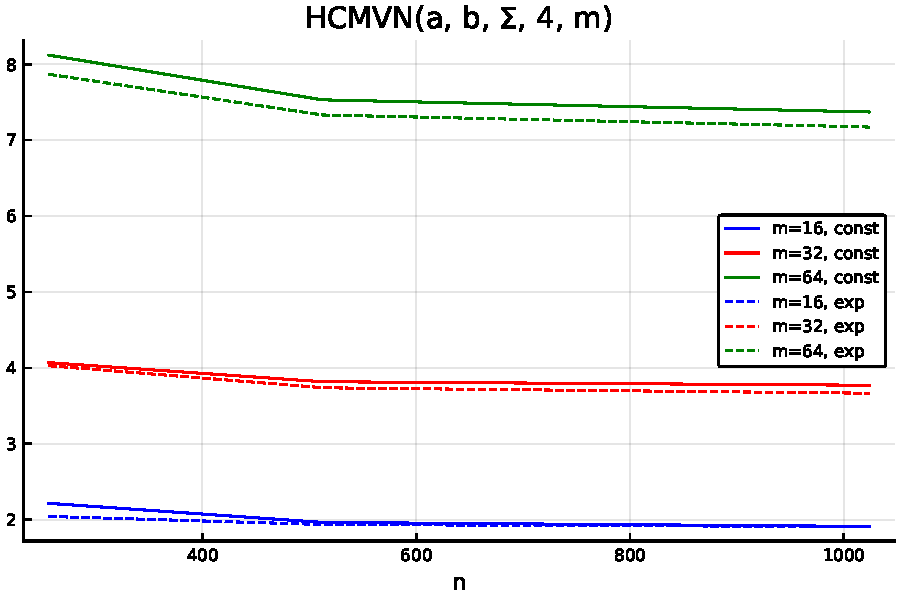
\includegraphics[width=\linewidth]{figs/table3_m2.pdf}
						\caption{\texttt{HCMVN}}
				\end{subfigure}\hfill
				\begin{subfigure}[b]{0.45\textwidth}
						\centering
						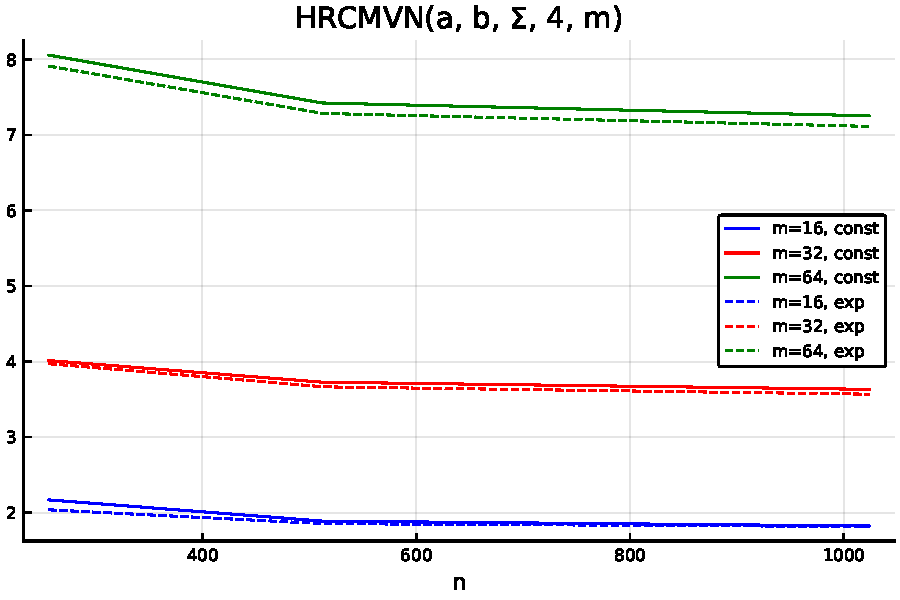
\includegraphics[width=\linewidth]{figs/table3_m3.pdf}
						\caption{\texttt{HRCMVN}}
				\end{subfigure}
		\caption{Execution time (seconds) for the hierarchical-block conditioning approximation}\label{fig:table3_hctime}
	\end{figure}	

	% The excution times of \texttt{HCMVN} and \texttt{HRCMVN} are significantly smaller than of \texttt{HMVN} even their performances are similar 

\end{frame}
\section{Elements}

\begin{frame}[fragile]{Typography}
      \begin{verbatim}The theme provides sensible defaults to
\emph{emphasize} text, \alert{accent} parts
or show \textbf{bold} results.\end{verbatim}

  \begin{center}becomes\end{center}

  The theme provides sensible defaults to \emph{emphasize} text,
  \alert{accent} parts or show \textbf{bold} results.
\end{frame}

\begin{frame}{Font feature test}
  \begin{itemize}
    \item Regular
    \item \textit{Italic}
    \item \textsc{SmallCaps}
    \item \textbf{Bold}
    \item \textbf{\textit{Bold Italic}}
    \item \textbf{\textsc{Bold SmallCaps}}
    \item \texttt{Monospace}
    \item \texttt{\textit{Monospace Italic}}
    \item \texttt{\textbf{Monospace Bold}}
    \item \texttt{\textbf{\textit{Monospace Bold Italic}}}
  \end{itemize}
\end{frame}

\begin{frame}{Lists}
  \begin{columns}[T,onlytextwidth]
    \column{0.33\textwidth}
      Items
      \begin{itemize}
        \item Milk \item Eggs \item Potatos
      \end{itemize}

    \column{0.33\textwidth}
      Enumerations
      \begin{enumerate}
        \item First, \item Second and \item Last.
      \end{enumerate}

    \column{0.33\textwidth}
      Descriptions
      \begin{description}
        \item[PowerPoint] Meeh. \item[Beamer] Yeeeha.
      \end{description}
  \end{columns}
\end{frame}
\begin{frame}{Animation}
  \begin{itemize}[<+- | alert@+>]
    \item \alert<4>{This is\only<4>{ really} important}
    \item Now this
    \item And now this
  \end{itemize}
\end{frame}
\begin{frame}{Figures}
  \begin{figure}
    \newcounter{density}
    \setcounter{density}{20}
    \begin{tikzpicture}
      \def\couleur{alerted text.fg}
      \path[coordinate] (0,0)  coordinate(A)
                  ++( 90:5cm) coordinate(B)
                  ++(0:5cm) coordinate(C)
                  ++(-90:5cm) coordinate(D);
      \draw[fill=\couleur!\thedensity] (A) -- (B) -- (C) --(D) -- cycle;
      \foreach \x in {1,...,40}{%
          \pgfmathsetcounter{density}{\thedensity+20}
          \setcounter{density}{\thedensity}
          \path[coordinate] coordinate(X) at (A){};
          \path[coordinate] (A) -- (B) coordinate[pos=.10](A)
                              -- (C) coordinate[pos=.10](B)
                              -- (D) coordinate[pos=.10](C)
                              -- (X) coordinate[pos=.10](D);
          \draw[fill=\couleur!\thedensity] (A)--(B)--(C)-- (D) -- cycle;
      }
    \end{tikzpicture}
    \caption{Rotated square from
    \href{http://www.texample.net/tikz/examples/rotated-polygons/}{texample.net}.}
  \end{figure}
\end{frame}
\begin{frame}{Tables}
  \begin{table}
    \caption{Largest cities in the world (source: Wikipedia)}
    \begin{tabular}{lr}
      \toprule
      City & Population\\
      \midrule
      Mexico City & 20,116,842\\
      Shanghai & 19,210,000\\
      Peking & 15,796,450\\
      Istanbul & 14,160,467\\
      \bottomrule
    \end{tabular}
  \end{table}
\end{frame}
\begin{frame}{Blocks}
  Three different block environments are pre-defined and may be styled with an
  optional background color.

  \begin{columns}[T,onlytextwidth]
    \column{0.5\textwidth}
      \begin{block}{Default}
        Block content.
      \end{block}

      \begin{alertblock}{Alert}
        Block content.
      \end{alertblock}

      \begin{exampleblock}{Example}
        Block content.
      \end{exampleblock}

    \column{0.5\textwidth}

      \metroset{block=fill}

      \begin{block}{Default}
        Block content.
      \end{block}

      \begin{alertblock}{Alert}
        Block content.
      \end{alertblock}

      \begin{exampleblock}{Example}
        Block content.
      \end{exampleblock}

  \end{columns}
\end{frame}
\begin{frame}{Math}
  \begin{equation*}
    e = \lim_{n\to \infty} \left(1 + \frac{1}{n}\right)^n
  \end{equation*}
\end{frame}
\begin{frame}{Line plots}
  \begin{figure}
    \begin{tikzpicture}
      \begin{axis}[
        mlineplot,
        width=0.9\textwidth,
        height=6cm,
      ]

        \addplot {sin(deg(x))};
        \addplot+[samples=100] {sin(deg(2*x))};

      \end{axis}
    \end{tikzpicture}
  \end{figure}
\end{frame}
\begin{frame}{Bar charts}
  \begin{figure}
    \begin{tikzpicture}
      \begin{axis}[
        mbarplot,
        xlabel={Foo},
        ylabel={Bar},
        width=0.9\textwidth,
        height=6cm,
      ]

      \addplot plot coordinates {(1, 20) (2, 25) (3, 22.4) (4, 12.4)};
      \addplot plot coordinates {(1, 18) (2, 24) (3, 23.5) (4, 13.2)};
      \addplot plot coordinates {(1, 10) (2, 19) (3, 25) (4, 15.2)};

      \legend{lorem, ipsum, dolor}

      \end{axis}
    \end{tikzpicture}
  \end{figure}
\end{frame}
\begin{frame}{Quotes}
  \begin{quote}
    Veni, Vidi, Vici
  \end{quote}
\end{frame}

{%
\setbeamertemplate{frame footer}{My custom footer}
\begin{frame}[fragile]{Frame footer}
    \themename defines a custom beamer template to add a text to the footer. It can be set via
    \begin{verbatim}\setbeamertemplate{frame footer}{My custom footer}\end{verbatim}
\end{frame}
}

\begin{frame}{References}
  Some references to showcase [allowframebreaks] \cite{knuth92,ConcreteMath,Simpson,Er01,greenwade93}
\end{frame}

\section{Conclusion}

\begin{frame}{Summary}

  Get the source of this theme and the demo presentation from

  \begin{center}\url{github.com/matze/mtheme}\end{center}

  The theme \emph{itself} is licensed under a
  \href{http://creativecommons.org/licenses/by-sa/4.0/}{Creative Commons
  Attribution-ShareAlike 4.0 International License}.

  \begin{center}\ccbysa\end{center}

\end{frame}

{\setbeamercolor{palette primary}{fg=black, bg=yellow}
\begin{frame}[standout]
  Questions?
\end{frame}
}

\appendix

\begin{frame}[fragile]{Backup slides}
  Sometimes, it is useful to add slides at the end of your presentation to
  refer to during audience questions.

  The best way to do this is to include the \verb|appendixnumberbeamer|
  package in your preamble and call \verb|\appendix| before your backup slides.

  \themename will automatically turn off slide numbering and progress bars for
  slides in the appendix.
\end{frame}

\begin{frame}[allowframebreaks]{References}
  
  \bibliographystyle{apalike} % apa style
  \bibliography{refs}

\end{frame}

\end{document}
